
%%%%%%%%%%%%%%%%%%%%%%% file typeinst.tex %%%%%%%%%%%%%%%%%%%%%%%%%
%
% This is the LaTeX source for the instructions to authors using
% the LaTeX document class 'llncs.cls' for contributions to
% the Lecture Notes in Computer Sciences series.
% http://www.springer.com/lncs       Springer Heidelberg 2006/05/04
%
% It may be used as a template for your own input - copy it
% to a new file with a new name and use it as the basis
% for your article.
%
% NB: the document class 'llncs' has its own and detailed documentation, see
% ftp://ftp.springer.de/data/pubftp/pub/tex/latex/llncs/latex2e/llncsdoc.pdf
%
%%%%%%%%%%%%%%%%%%%%%%%%%%%%%%%%%%%%%%%%%%%%%%%%%%%%%%%%%%%%%%%%%%%


\documentclass[runningheads,a4paper]{llncs}

\usepackage{amssymb}
\setcounter{tocdepth}{3}
\usepackage{graphicx}
\usepackage[nolist]{acronym}

%\usepackage{hyphenat} see
%http://www.ctan.org/tex-archive/macros/latex/contrib/hyphenat - would
%be good to enable this to prevent hyphenation of OWL MS statements.
%Or find alternative

\usepackage{url}
\usepackage{tabularx}
\newcolumntype{Y}{>{\centering\arraybackslash}X}
\usepackage{makecell}
%\urldef{\mailsa}\path|davidos@ebi.ac.uk|

\newcommand{\keywords}[1]{\par\addvspace\baselineskip
\noindent\keywordname\enspace\ignorespaces#1}

\def\correspondingauthor{$^*$}
\def\@corresponding{\footnotesize\correspondingauthor Corresponding author} 


\begin{document}

\mainmatter  % start of an individual contribution

% first the title is needed
\title{Cell, chemical and anatomical views of the Gene Ontology: mapping to a Roche controlled vocabulary.}

% a short form should be given in case it is too long for the running head
\titlerunning{Cell, chemical and anatomical views of the Gene Ontology.}

% the name(s) of the author(s) follow(s) next
%
% NB: Chinese authors should write their first names(s) in front of
% their surnames. This ensures that the names appear correctly in
% the running heads and the author index.
%
\author{David Osumi-Sutherland$^1*$, Enrico Ponta$^2$, Melanie Courtot$^1$ and Helen Parkinson$^1$, Laura Badi$^2$}  % TBC

%
\authorrunning{Cell, chemical and anatomical views of the Gene Ontology.}
% (feature abused for this document to repeat the title also on left hand pages)

% the affiliations are given next; don't give your e-mail address
% unless you accept that it will be published
\institute{$^1$ European Bioinformatics Institute (EMBL-EBI), European Molecular Biology Laboratory, Wellcome Trust Genome Campus, Hinxton, Cambridge CB10 1SD, United Kingdom \\
$^2$ F. Hoffmann-La Roche Ltd
Grenzacherstrasse 124, CH-4070 Basel, Switzerland }
%* corresponding author: davidos@ebi.ac.uk

% \mailsa\\  % This needs to be fixed!

%
% NB: a more complex sample for affiliations and the mapping to the
% corresponding authors can be found in the file "llncs.dem"
% (search for the string "\mainmatter" where a contribution starts).
% "llncs.dem" accompanies the document class "llncs.cls".
%

\toctitle{}
\tocauthor{}
\maketitle

\begin{abstract}

The Gene Ontology (GO) consists of around 40,000 terms for biological processes, cell parts and gene product activities. It has been used to annotate the functions of millions of gene products. Much pharmacological research focuses on understanding how disease conditions differ from physiological conditions in molecular terms with the aim of finding new drug targets for therapy. Gene-set enrichment analysis (GSEA) using the Gene Ontology (GO) and its annotations, provides a powerful way to assess those differences 

Roche has developed a bespoke controlled vocabulary (RCV) to support enrichment analysis to a set of concepts that are important to its research aims. RCV includes terms for concepts that are not found in the GO, such as cell types, anatomical structures. Each term is manually mapped to a list of \ac{GO} terms. This manual mapping strategy is labour intensive and hard to sustain as the GO evolves. 

In this paper we describe the automation of mappings between RCV and the GO via OWL-EL queries, making use of extensive axiomatisation that links the GO to ontologies of cell type, anatomy and chemicals. We can fully automate mapping for about a third of the terms in the RCV, with another third having 5 or fewer GO terms requiring manual mapping. We show how a dataset analyzed using the RCV highlights the main processes affected by the perturbation in a compact fashion, allowing easy classification at-a-glance of result hits by visualization tools. 

The OWL query approach described here has potential for providing many new ways to query the GO, group annotations and carry out gene set enrichment analyses. 

\keywords{OWL, OWL-EL, controlled vocabulary}
\end{abstract}

\section{Introduction}

The \acf{GO} is widely used to annotate and group gene products according to their subcellular location (e.g., endoplasmic reticulum), molecular function (e.g., enzyme activity) and their wider role in cellular, developmental and physiological processes (e.g., signal transduction) {\cite{GO2015}). The logical structure of the ontology is used to group genes annotated with related terms in user facing tools such as QuickGO () and Amigo () and for gene-set enrichment analysis (GSEA) \cite{Merico2010} %\cite{Blake2015} - Helen want Best practice ref in here.  Having trouble finding.
, a technique for determining the over- or under-representation of general classes of gene products in experimental datasets. Grouping and GSEA typically only use logical relationships \textit{within} each of the 3 sub-ontologies of the \ac{GO} - cellular component, molecular function and biological process.  GSEA typically makes use of a slim version of the GO - including only a subset of high or intermediate level GO classes with a level of specificity appropriate to the study.  Annotations to more specific classes in the GO are mapped up to classes in the slim via a subset of relationship types in the GO (typically is\_a and part\_of).

Much pharmacological research focuses on understanding of how disease conditions differ from physiological conditions in molecular terms with the aim of finding new drug targets for therapy. GSEA provides a fruitful way to find functionally coherent gene-sets, such as pathways, that are statistically over or under-represented in gene lists derived differential expression experiments analysing disease models or pathological tissue samples.  Roche maintains a controlled vocabulary (from here referred to as RCV) for use in GSEA.  RCV consists of around 360 terms, each of which is mapped to a list of terms from GO, just as a term in a GO slim maps to a list of subclasses and subparts. The set of concepts is tailored to the research interests of Roche and is chosen with the aim of achieving geneset composition that is descriptive and broad enough to allow robust and statistically significant results, though not so broad and redundant in composition that it prevents easy result interpretation.

Some of the terms in RCV refer to concepts that are represented by named classes in the GO (as in a GO slim), but many refer to concepts that are orthogonal to the classification structure of the GO, such as types of cell, tissue or chemical.  Detecting enrichment to anatomy, organ or cell-specific processes or components can be critical for pharmacological research, especially when working with complex tissues where there is a need to tease apart events occurring in specific tissue compartments or cell types. For example, one Roche use case involves analysing differential expression in tissues samples from controls \textit{vs} an animal model of ectopic cartilage formation associated with fibrosis.  For this use case, it is useful to look for enrichment under processes affecting or occurring in cartilage.

In recent years, \ac{GO} has switched its underlying formalization to Web Ontology Language (OWL2) (\url{http://www.w3.org/TR/owl2-primer/}), and has dramatically increased the number of logical axioms \cite{Mungall2014}. This new axiomatisation includes many new relationship types, relationships between terms in different \ac{GO} sub-ontologies and extensive logical links to terms from external ontologies including the cell ontology \cite{Meehan2011}, the chemical ontology ChEBI {\cite{Hastings2013} and the Uberon multi-species anatomy ontology \cite{Haendel2014}.  For example, the chemical participants in over 12,000 processes or functions are specified in \ac{GO} via axioms referencing chemical entities defined by ChEBI \cite{Hill2013}. Over 8000 \ac{GO} classes have some direct or indirect logical link to a term from the Cell ontology or Uberon. These record, for example, the location of cellular components (e.g., the acrosome and its parts are present only in sperm), cell types that are the sole location of some process (e.g., 'natural killer cell degranulation' only occurs in natural killer cells ), and the products of developmental processes (e.g., bone is a product of 'bone morphogenesis').

Axiomatisation of the \ac{GO} is limited to the EL profile of OWL \cite{Mungall2014}. This allows \ac{GO} infrastructure to take advantage of fast, scalable OWL-EL reasoners such as ELK \cite{kazakov2012} to leverage the classifications in external ontologies to automate classification in \ac{GO}, and to ensure that classification and querying of the \ac{GO} will not become intractable as the ontology grows.  This axiomatisation also makes it possible to construct bespoke classifications of GO classes and their annotations that are orthogonal to the classification axes of the GO. For example, we can use OWL queries to group genes involved in processes occurring in T-cells or in the pancreas, or to group annotations to genes involved in the processes involving nitric oxide.

To date, each RCV term has been manually mapped to a list of GO terms on the basis of the lexical content of the names of \ac{GO} terms and the biological knowledge of those doing the mapping.  Keeping this mapping up to date and complete has become impractical given the evolution of the \ac{GO}.  Here we describe the development and testing of an automated mapping between \ac{GO} and RCV, making use of OWL reasoning to logically specify lists of GO classses subsumed by concepts referred to by RCV terms.

\section{Methods}

RCV is a flat list and includes concepts that are orthogonal to the axes of classification in the \ac{GO}. It is therefore not amenable to mapping via standard ontology alignment techniques. %poss ontlogy alignemt ref here?
  However, its relatively small size makes it viable to manually map each concept to a GO class expression, which can then be used in conjunction with an OWL reasoner to generate lists of terms GO terms subsumed by the RCV concept. For the purposes of automated mapping, we interpret the manually mapped \ac{GO} terms as subclasses of the class referred to by the RCV term. RCV does not include textual defintions, so for each RCV term, we attempted to find a class expression (a mapping query) that reflected the intended meaning of the RCV term, as judged by the RCV term name and manual mappings and based on discussion with Roche.

\subsection{Pipeline}

Mapping queries were run using the ELK OWL reasoner \cite{kazakov2012} via calls to the OWL-API \cite{Horridge2011}.  The query and results processing pipeline was written in Jython, a Python implementation over Java (\url{http://www.jython.org/}).  All code, mapping tables and results for the pipeline were maintained in a GitHub repository (\url{https://github.com/GO-ROCHE-COLLAB/Roche_CV_mapping}). 

The mapping was specified using a single TSV file in which each line maps an RCV term to an OWL-EL mapping query including a term from \ac{GO}, ChEBI, CL, Uberon or NCBI taxonomy.  The results of running each query resulted in a list of automated mappings from RCV to GO. Standard GitHub tickets were generated by script for all RCV terms mapped, with each ticket linked to a results table in tsv format allowing direct comparison of manual and automated mappings (see figure \ref{tab:mapping_table} for an example).  These files, which are automatically displayed on GitHub as tables, were manually reviewed and edited by RCV curators at Roche who used the linked tickets to discuss mapping issues and record the approval status of all mappings.

\subsection{Query strategy}

We chose to restrict mapping queries to the EL profile of OWL2, allowing us to use the fast, scaleable EL reasoner, ELK to run queries \cite{kazakov2012}.  This ensures that the mapping strategy will remain viable even if future versions of the GO become intractable to classification by fully expressive OWL DL reasoners. In order to keep the mapping process simple, we added a further restriction: only a single mapping class was specified for each mapping.

To compensate partially for the lack of disjunction (OR) in OWL-EL, we developed a heirarchy of high level object properties for use in queries. For example, we define \textbf{occurs\_in\_OR\_has\_participant} as a grouping relation allowing queries for processes that occur in a specified cell, or have that cell as a participant. \ac{GO} does not use a reflexive relation for 'part of', but using one for query purposes means a query for subclasses of  ``'part of' some X" returns both subclasses and proper parts of class X. Many RCV terms group processes in which a specified chemical or cell participates, with processes regulating those in which it participates (see Table 1 for example). To support such groupings, we used an OWL property chain axiom (\url{http://www.w3.org/TR/owl2-primer/#Property_Chains}) to define a relation, \textbf{regulates\_o\_has\_participant}, to query for processes that regulate a process in which some specified entity is a participant. We then define a super-property, \textbf{participant\_OR\_reg\_participant}, for this new relation and \textbf{has\_participant}

\begin{quote} % install /nohyphens for this?
\textbf{regulates} \textit{o} \textbf{has\_participant} \textit{subPropertyOf} \textbf{participant\_OR\_reg\_participant}

\textbf{regulates\_o\_has\_participant} \textit{subPropertyOf} \textbf{participant\_OR\_reg\_participant}

\textbf{has\_participant} \textit{subPropertyOf} \textbf{participant\_OR\_reg\_participant}
\end{quote}


The heavy use of OWL Object Property axioms to compensate for loss of expressivity tends to obscure the semantics of mappings. In order to record and communicate the meanings of mappings clearly, we used a script to generate human readable descriptions for each mapping query.  For example, we mapped the RCV term cannabinoid to the OWL query: \textbf{participant\_OR\_reg\_participant \textit{some} cannabinoid (CHEBI:67194)  }.  The automated description of the mapping reads:  ``A process in which a cannabinoid participates, or that regulates a process in which a cannabinoid participates."

\begin{table}
 \caption{Example mapping table.}
      \label{tab:mapping}
      \caption{\textbf{Results table for RCV cannabinoid.}  The table shows a comparison of the manual mapping of RCV to \ac{GO} terms (manual column) with the automated mappings (auto column) resulting from the an OWL query for processes with a cannabinoid as a participant and regulators of those processes. The automated mapping found three additional GO terms compared to the manual mapping. In this case, no manually mapped terms were obsolete in GO in this case, and all automated mappings were approved.}
      \begin{tabularx}{\textwidth}{@{}| c | c|Y|Y|Y|Y|Y|@{}}
        \hline
        \textbf{name}&\textbf{ID}&\textbf{manual}&\textbf{auto}&\textbf{checked}&\textbf{\thead{black\\listed}}&\textbf{\thead{is\\obsolete}} \\ \hline 
        \thead{regulation of \\ endocannabinoid \\ signaling pathway}&\ac{GO}\_2000124&1&1&1&0&0 \\ \hline
        \thead{cannabinoid \\signaling pathway}&\ac{GO}\_0038171&1&1&1&0&0 \\ \hline
        \thead{endocannabinoid \\signaling pathway}&\ac{GO}\_0071926&1&1&0&0&0 \\ \hline
        \thead{cannabinoid \\receptor activity}&\ac{GO}\_0004949&0&1&1&0&0 \\ \hline
       \thead{ cannabinoid \\biosynthetic process}&\ac{GO}\_1901696&0&1&1&0&0 \\ \hline
        \end{tabularx}
 \end{table}


\subsection{Gene set enrichement analyses} 

Expression of genes was measured in 2 conditions ( A and B ) and signals for individual genes were compared. Genes were ranked from the most highly changed in condition B vs condition A (positively changed) to the most negatively changed (negatively changed). After ranking, GSEA enrichment scores were computed, resulting in a list of geneset hits which were perturbed in condition B as opposed to condition A.  The results were analysed using the Enrichment Map software \cite{Merico2010} which provides a graphical representation of enrichment results.
 %Needs more details of how the analysis was done.  What software?  What cutoffs?


\section{Results}

Mapping followed an iterative process.  First mapping queries were selected and tested: subclasses of the mapping query (hereafter referred to as automated mappings) were reviewed against manual mappings to decide which patterns were most appropriate.  Once a mapping query was chosen, corrections and/or additions to the GO were made where results were wrong or incomplete.  At this point, any clear errors in the manual mapping were blacklisted. Review of automated mappings was then passed to Roche who approved or blacklisted individual classes. When satisfied with the results, the corresponding GitHub ticket was closed, thereby indicating the mapping as approved (see Table \ref{tab:mapping}  for an example).  Roche approved results were combined to produce a new RCV mapping table with a similar format to the original RCV mapping.  They were also used to generate an OWL file of RCV terms, importing GO and including automated textual definitions. 

\subsection{Mapping results}

We developed successful, Roche approved mapping queries for 308/364 RCV term.  Over a third (104) of the mapping queries were sufficient - meaning that no manual maintenance is required - and a further third of the mappings (148) had 10 or fewer additional manual mappings (Figure \ref{fig:man_only}). 
 
\begin{figure}
\centering
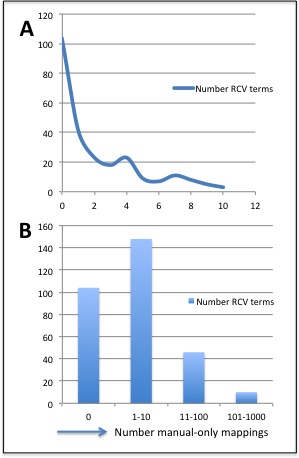
\includegraphics[width=70mm]{man_only.png}
\caption{\textbf{Distribution of manual only mappings.} A: Number of terms (Y-axis) vs number of manual mappings (X-axis) (cut-off at 20 manual mappings). 1B: Distribution of manual only mapping: 104 terms have no manual-mappings at all.  A further 148 have between 1 and 10.  The largest number of manual-only mappings for a single RCV terms was 323}
\label{fig:man_only}
\end{figure}
 
Mapping queries found many \ac{GO} terms that were not in the manual mapping, as shown on Figure \ref{fig:auto_only}.  For a few very general RCV classes (e.g., enzyme), over 1000 new mappings were found. Very few automated mappings were blacklisted - just 70 terms in total.  Blacklisting of terms ensured they were removed from the final mapping.

\begin{figure}
\centering
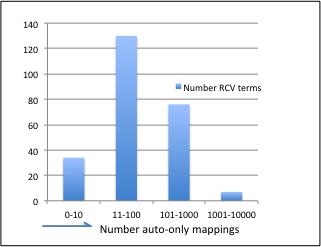
\includegraphics[width=70mm]{auto_only.png}
\caption{\textbf{Distribution of auto only mappings.}
X axis = number of auto-only mappings.  Y axis = Number of RCV terms.  Most mapping queries found under 100 additional (auto only) mappings, but over 75 found between 101 and 1000 and a few mapping queries found between 1001 and 10000 new mappings.}
\label{fig:auto_only}
\end{figure}

56 terms were not mapped.  Some were rejected from the pipeline as they were judged to be duplicates with other RCV terms.  The rest were rejected as currently unmappable due to the lack of suitable terms or axiomatisation within the \ac{GO} at this time.  For example, \ac{GO} currently has no way to group aerobic or anaerobic metabolic processes, although it does reflect the aerobic or anaerobic nature of many metabolic processes in their names and textual definitions. Further formalisation of the \ac{GO} is likely to improve the number of concepts that can be mapped.

\subsection{Testing the implication of automated mapping for gene set enrichment analyses}

The main use of RCV by Roche is in gene set enrichment analyses.  We tested the new RCV by carrying out a GSEA on a differential expression a dataset from Roche. %How many details can we add??}. 

Results were visualised using graphs produced by Enrichment Map \cite{Merico2010}.  Clustered nodes linked by edges indicate enrichment to muliple nodes.

A standard GO slim produces a usable result, doesn't have many concepts most needed by Roche (fig \ref{fig:GSEA}A).  The original, manual RCV-GO mapping results produces sparse, disconnected gene sets with very little redundancy (fig \ref{fig:GSEA}B).  The new, partially automated RCV-GO mapping results in enrichment to clusters of related gene sets, with many enrichment results not found in by the original mapping (fig \ref{fig:GSEA}C}.  The difference in results is likely due to the new mapping being much more complete than the original.  The redundancy between gene sets is not so great as to obscure the results and is actually potentially informative.  Some of this redundancy is due to mapping of GO terms to multiple classes.  For example the RCV classes `heart function' and `ion channel activity' have N GO terms in common.  In other cases, for example RCV:glutamatergic and RCV:behavior, clustering occurs where there are no GO terms in common, and must be due to annotation of the same gene or genes to both concepts.  In both cases the link between the concepts makes biological sense.

% 1. Shouldn't we be comparing to a standard slim rather than to all of BP
% 2. Surely some redundancy must be useful.  It shows potential connections between processes or between functions and processes:  particular ion channels in heart function for example.  Shouldn't we emhasise this.
% 3. Perhaps should zoom in on some set of connected, enriched terms for discussion?

% NOTE _ CURRENT FIG IS PLACEHOLDER until we get higher res one + analysis repeated with generic goslim.
\begin{figure}
\centering
\caption{A graphical representation of GSEA using manual mapping from RCV to GO (panel A) vs semi-automated mapping (panel B).  Red nodes show postitively enriched gene sets.  Blue nodes show negatively enriched. The size of the node is proportional to the geneset size and the connecting edge thickness is a measure of the mutual relationship among 2 gene sets in terms of redundancy.}
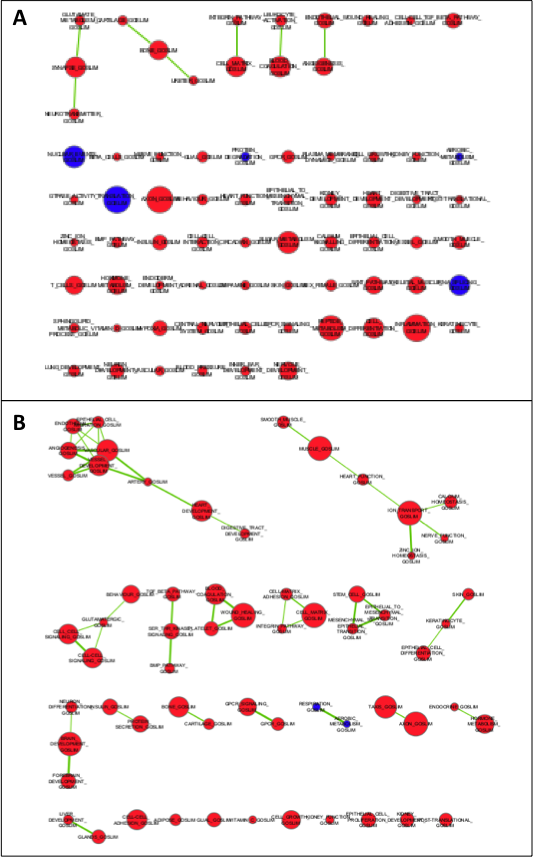
\includegraphics[width=120mm]{GSEA.png}
\label{fig:GSEA}
\end{figure}


\subsection{Improvements to the GO}

GO has extensive axiomatisation linking processes to cells, anatomical structures and chemicals, but this is not always complete.  In mapping from RCV to GO we found and corrected over 200 omissions in the axiomatisation.  This included missing links from processes to participant cell types, anatomical structures, chemicals and cell components and transcript types.  We also found and corrected a number of errors in axiomatisation, including axiomatisation of developmental processea that lead to incorrect inferences for RCV anatomy terms.

% Examples: 
% * Fixed dodgy inference of gastrulation as subclassof disgestive   tract morphogenesis (and therefore part of dt development) (Revision 23125)
% * Incorrect (reversed) classifications relating to skin & epidemis development development (Revision 22950)


\section{Discussion and future directions}

This work demonstrates how the logical structure of the \ac{GO} can be used to achieve biologically meaningful mappings between \ac{GO} and terms from external controlled vocabularies or ontologies for which there is no corresponding \ac{GO} term.  For example, where the external vocabulary refers to a cell-type, a chemical or an anatomical structure.  The mapping system used is fast and scalable,  but a few improvements would be beneficial.

%Dic
\subsection{Improving the RCV mapping pathway}

There is good scope for improving the mapping between RCV and \ac{GO} so that it is more thoroughly automated. 

We are currently reviewing RCV terms with only a small number of additional manual mappings in order to decide whether the overhead of manual maintenance is worth the effort, especially where these additional mappings could not be achieved by further axiomatisation of the \ac{GO}.  For example, mappings to cell types often include mappings to growth factors acting on those cell types.  As these growth factors have much broader functions than action on the cell types for which they are named, \ac{GO} is unable to add any formal link between factors and cell types.

In other cases a mapping pattern involving two or more specified classes and a more sophisticated logic would be necessary to obtain a complete mapping.  For example, the manual mappings for X metabolism terms are consistently mapping to bot X metabolism and X transport terms in the \ac{GO}. A more complete mapping to RCV metabolism terms could be achieved using a pattern that named both \ac{GO} transport and \ac{GO} metabolic process terms.  This could be made scalable with a pipelines that combines the results of multiple mapping queries.  Although formal logic dictates that the results may be incomplete, this will not be an issue with the current GO axiomatisation.


\subsection{Alternative views of the \ac{GO} and its annotations}

The mechanisms described here for mapping to external ontologies could also be used for providing alternative views of the \ac{GO} and its annotations.  This is already reflected in some of the newer functionalities of the \ac{GO} browsing tool AMIGO, which now displayed inferred annotations to cell-types based on axioms in \ac{GO} recording where processes occur \footnote{http://amigo.geneontology.org/amigo/term/CL:0000084}.

\subsection{Future work}

The system described here was designed to be lightweight and flexible, allowing maximum interaction between the designers of RCV at Roche and \ac{GO} editors with minimal development overhead.

The pattern-based system used here bears some relationship to the TermGenie system \cite{Dietze2014} which is already used to generate 80\% of new \ac{GO} terms.  One possible approach to fulfilling the needs of external groups for types of classification not included in the \ac{GO} would be to offer a TermGenie-like system for generating terms that group \ac{GO} terms in ways that are not currently supported internally by the \ac{GO}.

%
%\subsection*{Author's contributions}
%
%
%\subsection*{Acknowledgments.}
%Authors wish to acknowledge collaborators in the GO consortium.

\subsubsection*{Funding}

This work was supported by direct funding from F. Hoffmann-La Roche Ltd.  The Gene Ontology Consortium is supported by a P41 grant from the National Human Genome Research Institute (NHGRI) [grant 5U41HG002273-14].

%\begin{thebibliography}{}

\bibliography{Roche_swat4ls_2015} % Bibliography file (usually '*.bib' )

\bibliographystyle{plain}

%\end{thebibliography}

%%%%%%%%%%%


%%%%%%%%%%%%%%%%%%%%%%%%%%%%%%%%%%%
%%                               %%
%% Figures                       %%
%%                               %%
%% NB: this is for captions and  %%
%% Titles. All graphics must be  %%
%% submitted separately and NOT  %%
%% included in the Tex document  %%
%%                               %%
%%%%%%%%%%%%%%%%%%%%%%%%%%%%%%%%%%%

%%
%% Do not use \listoffigures as most will included as separate files 



\begin{acronym}
\acro{OWL}{Web Ontology Language}
\acro{GO}{Gene Ontology}
\acro{OBI}{Ontology of Biomedical Investigations}
\acro{OBO}{Open Biomedical Ontologies}
\acro{BFO}{Basic Formal Ontology}
\acro{ChEBI}{Chemical Entities of Biological Interest}
\acro{Uberon}{Uber anatomy ontology}
\acro{CL}{Cell Ontology)

\end{acronym}


\end{document}
